\usepackage{tikz}
\usepackage[absolute,overlay]{textpos}
\usepackage{booktabs}
\usepackage{longtable}
\usepackage{array}
\usepackage{multirow}
\usepackage{wrapfig}
\usepackage{float}
\usepackage{colortbl}
\usepackage{pdflscape}
\usepackage{tabu}
\usepackage{threeparttable}
\usepackage{threeparttablex}
\usepackage[normalem]{ulem}
\usepackage{makecell}
\usepackage{xcolor}

% define new footline defination
\setbeamertemplate{footline}
{
    \leavevmode%
    \hbox{%
        \begin{beamercolorbox}[wd = .5\paperwidth, ht = 1ex, dp = 1ex, center]{author in head/foot}%
            Text in footer
        \end{beamercolorbox}%
        \begin{beamercolorbox}[wd = .5\paperwidth, ht = 1ex, dp = 1ex, center]{date in head/foot}%
            \insertframenumber{}
        \end{beamercolorbox}
    }%
    \vskip3pt%
}
% add footline defination to the beamer template
\addtobeamertemplate{footline}{\begin{center}\rule{0.6\paperwidth}{0.4pt}\end{center}\vspace*{-1ex}}{}

% % set titlepage in a TikZ node for modifications
\setbeamertemplate{title page}{
\tikz\node[opacity=0.3] {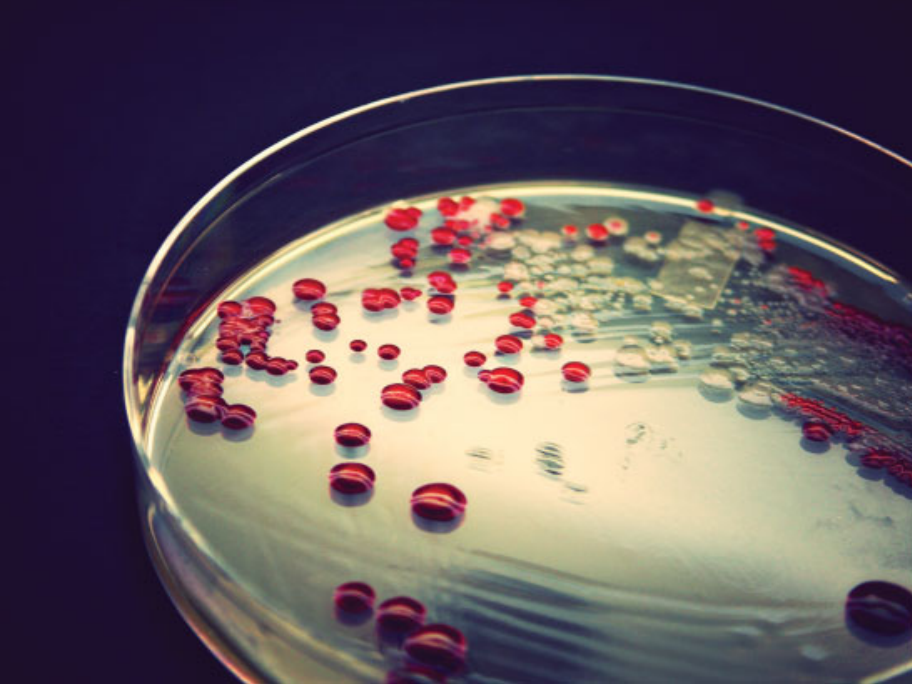
\includegraphics[height=\paperheight,width=\paperwidth]{03-gene_transfer_in_bacteria_bacterial_colony.png}};
% \tikz\node[opacity=0.8] {\includegraphics[width=5cm,ext=.1-overview_mutation_cover.png,type=png,read=.1-overview_mutation_cover.png]{1}} % if name shall contain dots, suppose filename = 01.1-overview_mutation_cover.png
\begin{textblock}{15}(1.5,2.8)\usebeamerfont{title} % 1.5 is x position in page
{\color{white}\raggedright\par\inserttitle}
\end{textblock}
\begin{textblock}{7.5}(1.5,7) % 1.5 is x position in page
{\color{white}\raggedright{\insertauthor}\mbox{}\\[0.2cm]
\insertdate}
\end{textblock}} % dd_rookie modified, figure is top aligned


% % set caption font size
% % note that beamer presentation native captions have their own configs
% \usepackage{caption}
% \captionsetup{font=footnotesize}

% this font option is amenable for beamer
\setbeamerfont{caption}{size=\tiny}

% some beamer themes naturally might not support navigation symbols
% \setbeamertemplate{navigation symbols}{} % remove navigation symbols

\setbeamertemplate{footline}[page number] % insert page number in footline
